\documentclass[12pt]{article}
\usepackage[T1]{fontenc}
\usepackage[utf8]{inputenc}
\usepackage[swedish]{babel}
\usepackage{geometry}
\usepackage{graphicx}
\usepackage{float}
\usepackage{amssymb}



\geometry{
  a4paper,
  total={170mm,257mm},
  left=20mm,
  top=20mm
}

\begin{document}

\setlength{\parindent}{0pt}
\section{Föreläsning 1}
\subsection{Att göra sin röst hörd som anställd}
\begin{itemize}
    \item Sorit ("exit") -- Att lämna organsationen
    \item Protest ("voice") -- Indivuellt eller kollektivt protestera mot hur ledningen agerar
    \item Lojalitet ("loyalty") -- Att stanna kvar och (passivt) acceptera ledningens hållning
\end{itemize}

\subsection{Reflektion}
\begin{itemize}
    \item Att approacha ett ämne på olika perspektiv 
    \item Att tillföra ett annat perspektiv
    \item Lika viktigt att lyssna som att tala
    \item Inte åsikter (rätt/fel) eller värderingar (bra/dåligt)
    \item Inte debatt
\end{itemize}

\subsection{De anställdas röst, olika paradigmer}
Employment relations (ER)
\begin{itemize}
    \item Beskriver hur aktörer med olika intressen interagerar med varandra
    \item Kollektivt perspektiv -- medbestämmande av arbetsprocesser
    \item Förhållandet påverkas av organsationen och institutioner genom exempelvis:
    \begin{itemize}
        \item Formella strukturer ger goda förutsättningar för att främja anställdas röst på anställdas villkor
        \item Ledningsstyrd röst tenderar att förekomma när där anställdas röst är svag
        \item Organisatorsiska förutsättning kan alltså öka eller minska sannolikheten att anställdas röst främjas
    \end{itemize}
    \item Fackföreningar är den vikigaste röstinstitutionen 
\end{itemize}

Organizational behavior (OB)
\begin{itemize}
    \item Beskriver hur individer och grupper beter sig
    \item Antangad: Ledningens och anställdas intresse ligger i linje med varandra
    \item Prosocialt beteene -- Anställda vill komma med förslag, ideer och förbättringar, ledningen lyssnar pga värdet för organisationen
    \item Icke värdeskapande uttryck är inte klagomål, missnöje är avgörande för anställdas röst
    \item Individuellt perspektiv -- anställda uttrycker sig på eget initiativ, inte kollektivt
    \item Perspektivet behandlar inte policies, regleringar eller strategiska frågor, utan fokuserar på individuella beteenden
\end{itemize}
\newpage
Human resource management (HRM)
\begin{itemize}
    \item Fokus på management och effektivt värdeskapande avv anställda
    \item Hur kan ledningen främja anställdas röst som förbättrar resultat?
    \item Skapa högpreseternade arbetsmetoder och HR-system 
    \item Direkt röst snarare än representativ röst genom:
    \begin{itemize}
        \item Hög autonomi
        \item Självstyrande team 
        \item Tillgång till kommunikationskanaler
    \end{itemize}
\end{itemize}

Labour process theory (LPT)
\begin{itemize}
    \item Anställdas röst som en del av en kamp mellan anställda och ledning
    \item Kritiskt perspektiv på olika intressen 
    \item Begränsad tro på att förena arbetstagare och ledningens intressen
\end{itemize}

Översikt:
\begin{figure}[H]
    \centering 
    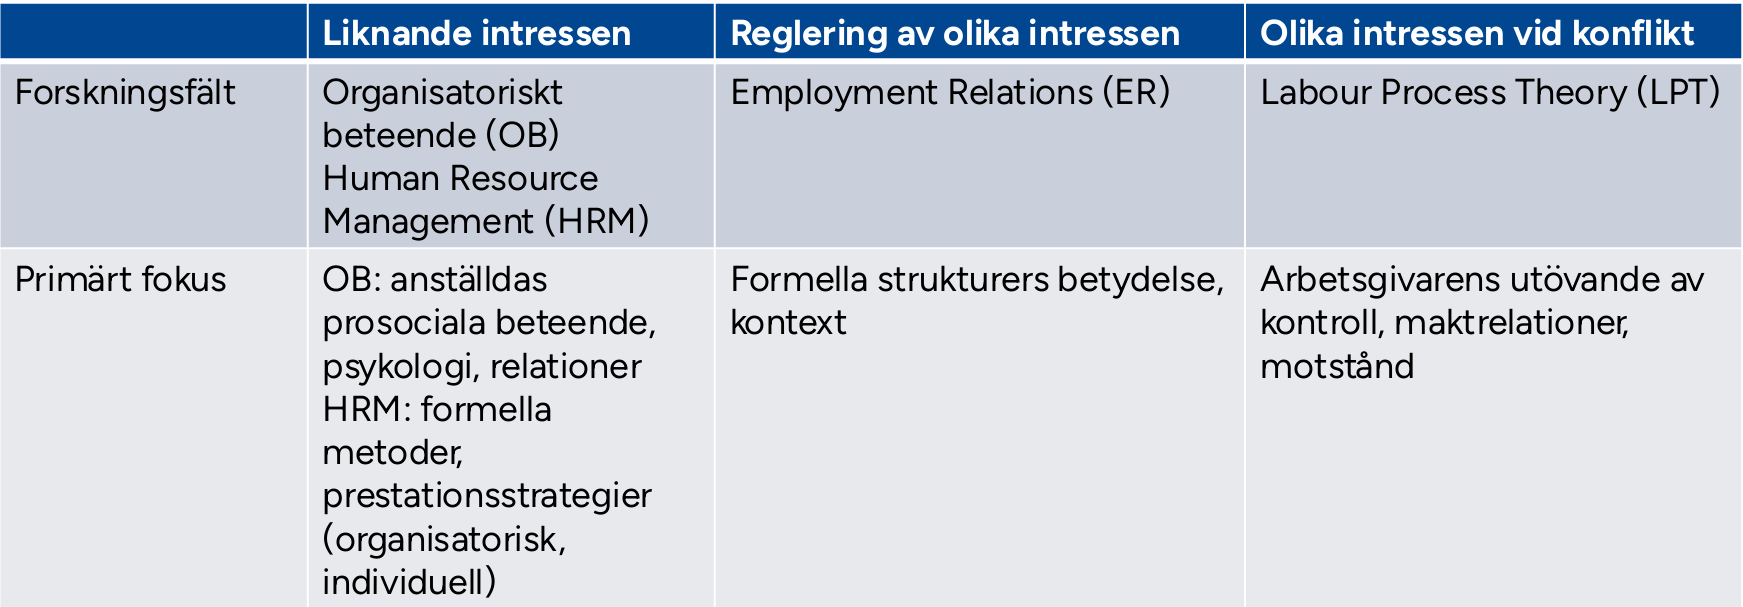
\includegraphics[width=0.8\textwidth]{paradigms.png}
\end{figure}

\subsection{Samarbete i arbetsrelationer}
\begin{itemize}
    \item Alla arbetsrelationer har samarbete, arbeta mot gemensamt mål
    \item Samarbete har en dualism mellan ömsesidighet och egenintresse
    \item Utgår ifrån ett framework i fem steg:
    \begin{enumerate}
        \item Vem/Vilka är samarbetar tillsammans?
        \item Går intressen att förena?
        \item Hur mycket ömsesidighet finns det?
        \item Hur kan ställda göra sin röst hörd?
        \item Vilka frågor samarbetar man kring?
    \end{enumerate}
\end{itemize}

\subsection{6 perspektiv på samarbete}
\begin{enumerate}
    \item Marknad/egoism -- Rationella aktörer som agerar utifrån individuellt egenintresse
    \item Autokratisk enhetssyn -- Arbetsgivare styr enväldigt för att uppnå organisatoriska mål vilket gynnar anställda
    \item Rådgivande enhetssyn -- Ledningen styr men är intresserad av anställdas behov och syn på organisatoriska mål
    \item Samarbetspluralism -- Fokus på gemensamma intressen och kompromissar kring motstridiga mål
    \item Motsättningspluralism -- Fokus på separata intressen och mål men kompromissar
    \item Kritisk/radikalt perspektiv -- Samarbete betyder påtvingad regelefterlevnad
\end{enumerate}

\subsection{Svenska arbetsmarknad: historisk utveckling}
\begin{enumerate}
    \item Decemberkompromissen 1906 -- Arbetsgivaren leder och fördelar arbetet, arbetstagarna har rätt att organisera sig i fackföreningar
    \item Kollektivavtalslagen 1928 -- Fredsplikt under kollektivavtalet
    \item Saltsjöbadsavtalet 1938 ("Den svenska modellen") -- Parterna kommer överens, ingen statlig inblandning
    \item 1970-talet LAS och MBL -- LAS: Lagen om anställningsskydd, MBL: Medbestämmandelagen och arbetstidslagen som reglerade arbetsiden till 40h/vecka
    \item Industriavtalet 1997 - Lönebildningen
    \item Huvudavtalet 2022 -- Föränderingar i LAS 
\end{enumerate}

\subsection{Regleringar i pyramidform}
\begin{enumerate}
    \item Basen -- Lagar: Anställningsskydd, semesterlagen, arbetstidslagen, diskrimineringslagen
    \item Mellan -- Centrala kollektivavtal: Ersättningar, löneavtal, lokal förhandlingsrätt
    \item Mellan -- Lokala kollektivavtal: Lokal anpassning av centrala avtal, exempelvis arbetstider, löneformer, kompetensutveckling
    \item Toppen -- Anställningsavtal: Individuella avtal, exempelvis anställningsform, lön, arbetstider
\end{enumerate}

\subsection{Samarbetspluralism i Sverige ("Den svenska modellen")}
Utmärkande för den svenska modellen:
\begin{itemize}
    \item Tidigt erkännande av förenings- och förhandlingsrätt
    \item Kollektivavtal -- instrument för arbetsfred och samhällsekonomisk balans
    \item Hög organisationsgrad
    \item Centralism -- makt/beslut koncentreras till en central ledning
    \item Kollektivt synsätt
\end{itemize}
Det är i första hand partnerna på arbetsmarknaden som genom förhandlingar ansvara för lönebildning och andra villkor i arbetslivet 

\subsection{Stridsåtgärder, sympatiåtgärder och lockout}
\begin{itemize}
    \item \textbf{Stridsåtgärder} -- Fackliga eller arbetsgivarledda påtryckningar e.g strejk, blockad eller lockout används vik konflikter
    \item Grundar sig konflikt från olika perspektiv: Lön, arbetsvillkor, arbetsmiljö, arbetstid, etc
    \item Parterna kan ta stridsåtgärder som påtryckningsmedel
    \item För parter som är budna och kollektivavtal gäller fredsplikt
    \item "Mjuka" stridsåtgärder -- Exempelvis nyanställningsblockad dvs. hindra arbetsgivaren att få ny arbetskraft
    \item \textbf{Sympatiåtgärder} -- Stridsåtgärder som vidtas i sympati med ett annat förbund
    \item \textbf{Lockout} -- Arbetsgivarnas motvapen till strejk
\end{itemize}

\subsection{Samarbetspluralism i Sverige}
\begin{itemize}
    \item Rätten till stridsåtgärder är grundlagsskyddad (kan inskränkas genom lag eller kollektivavtal)
    \item Avsaknad av kollektivavtal -- fritt att ta stridsåtgärder
    \item Partnerna har ansvar att åtgärderna inte medför "opåkallad skada" för tredje part
    \item Avtalsslutande organisation beslutat om åtgärden 
    \item Inga relger för proportionalitet
    \item Medling är det enda sättet för statlig inblandning
\end{itemize}

{\Huge $\Box$ }

\newpage

\section{Inför seminarium 1}
\subsection{Employees voice -- Barry et. al}
\subsection{Organizational behavior (OB)}
\begin{itemize}
    \item Röst ses som pro socialt beteende som gynnar organisationen
    \item Rösten är induviduellt och frivilligt initierat i syfte att hjälpa organisationen
\end{itemize}

\subsection{Human resource management (HRM)}
\begin{itemize}
    \item Betraktar röst som del av high-performance work practices (HPWP)
    \item Fokuserar på direkt istället för representativ röst
\end{itemize}

\subsection{Employer relation (ER)}
\begin{itemize}
    \item Förnekar pro social beteende ser röst som egenintresse
    \item Fokuserar på formella sturkturer och represenativ röst 
\end{itemize}

\subsection{Labor processtheory (LPT)}
\begin{itemize}
    \item Krtiskt perspektiv på röst som en kamp mellan anställda och ledning
    \item 
\end{itemize}

\subsection{Sammanvävning av perspektiv}
\begin{figure}[H]
    \centering 
    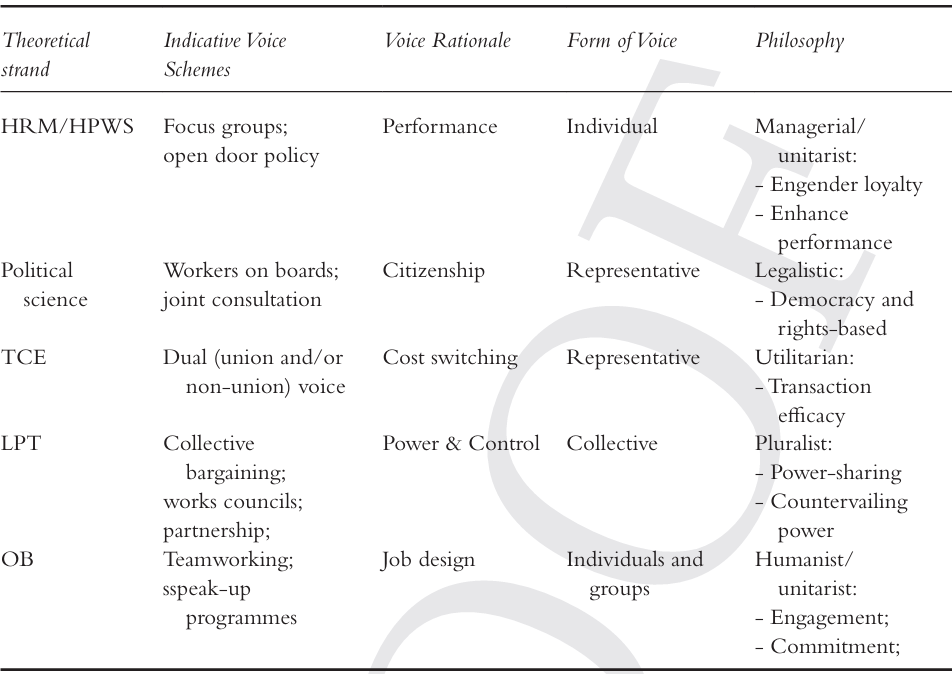
\includegraphics[width=0.8\textwidth]{perspectives.png}
\end{figure}

\begin{itemize}
    \item OB och HRM argumenterar att röst gynnar organisationen
    \item ER och LPT är mer kritiska och ser röst som en kamp mellan anställda och ledning
    \item OB förnekar helt att röst kan vara konfliktfyllt
    \item HRM erkänner att röst kan vara konflikt men fokuserar på att främja röst som gynnar organisationen
    \item OB tar inte hänsyn till instituionella och arbetsmiljömässiga faktorer
\end{itemize}

\subsection{Makt och röst}
\begin{itemize}
    \item OB har perspektivet att individer väljer att rösta eller vara tysta för att gagna organisationen
    \item ER vill anställda rösta för att få kontroll över organisations beslut de inte håller med om
\end{itemize}














\end{document}